% !TEX root = ../main.tex

\chapter{颗粒介质中的剪切带}

\section{引言}



\section{实验装置}

目前剪切装置和声学装置的耦合尚不成熟,因此只简要介绍有关于剪切装置的部分。图~\ref{fig:apparatus_2} 展示了剪切实验中的各部件。

\begin{figure}[!htp]
    \centering
    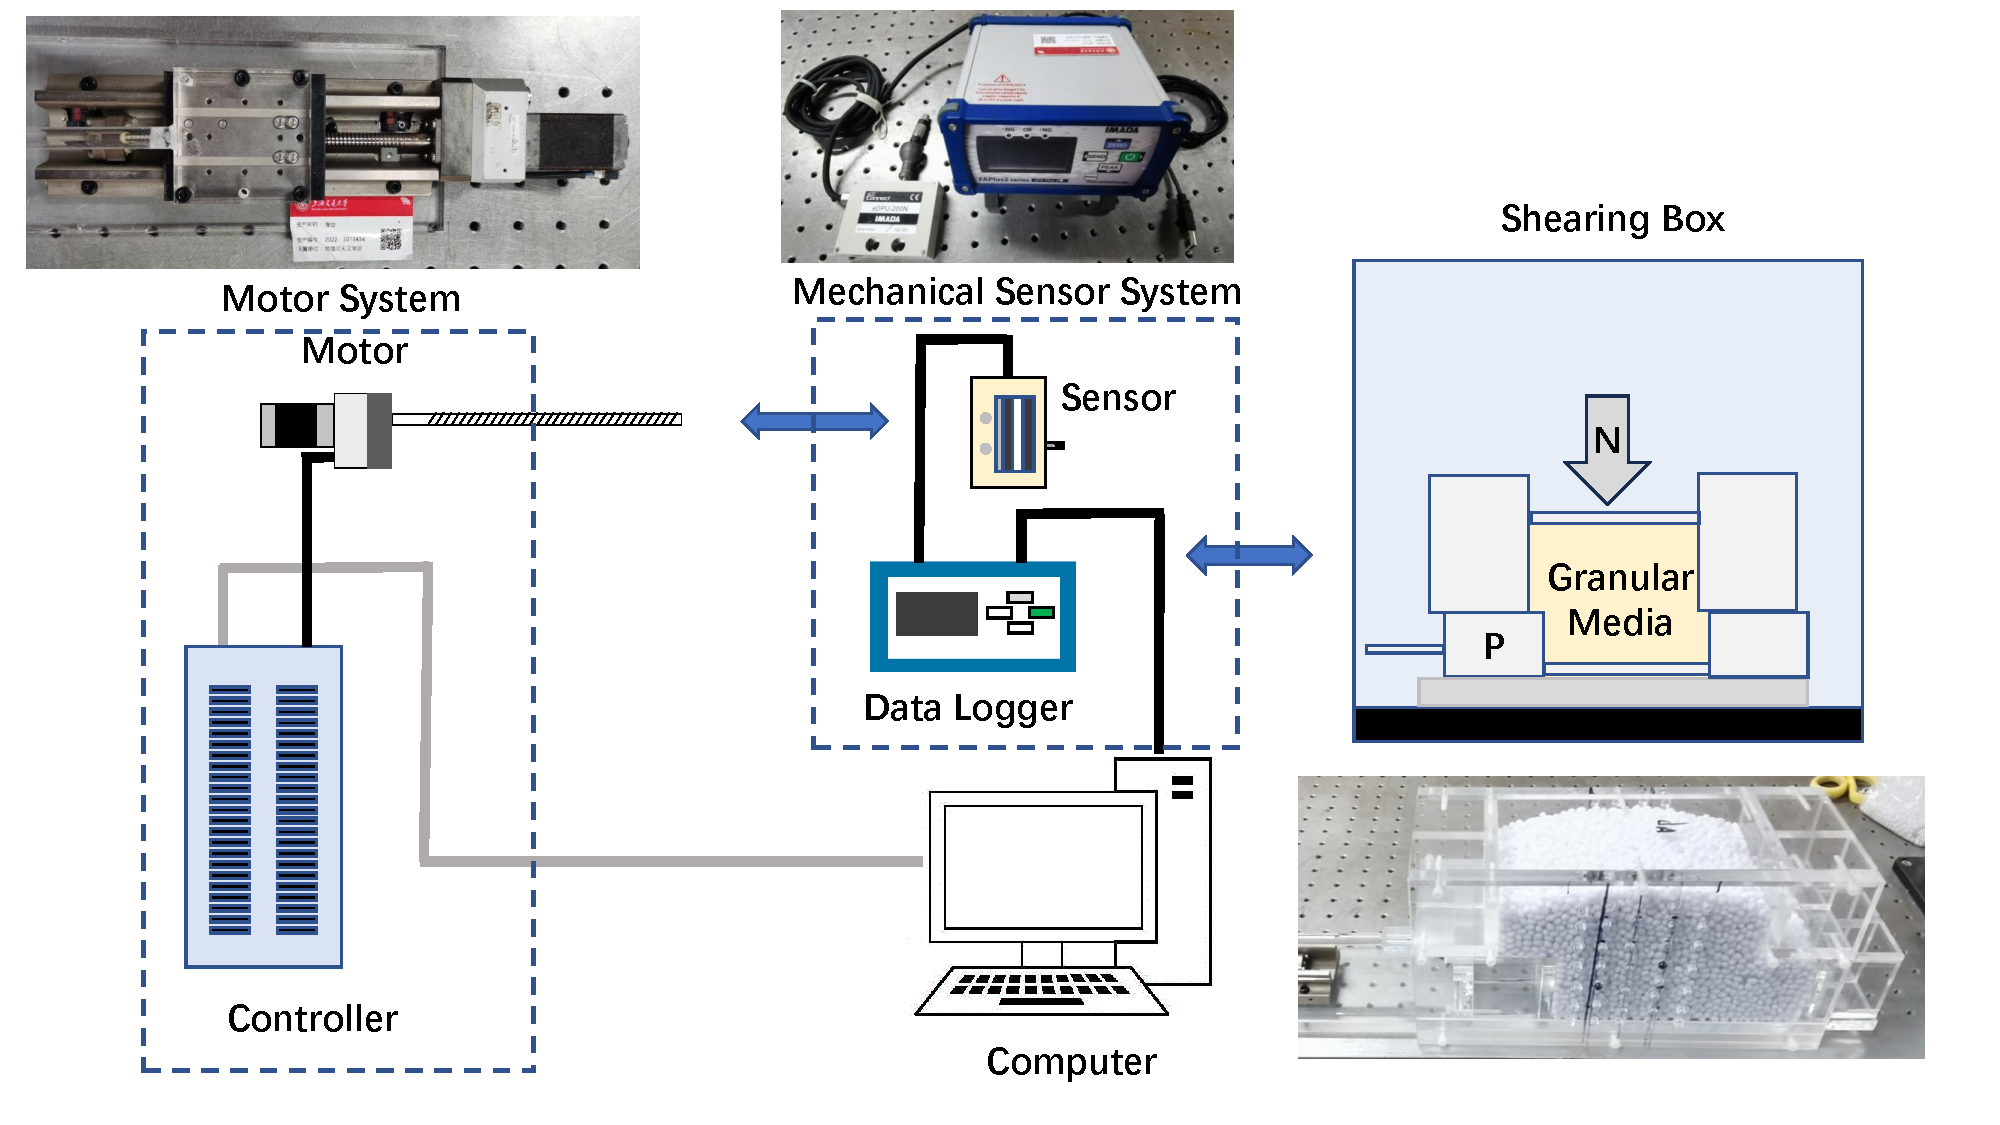
\includegraphics[height=8.5cm]{figures/4_apparatus.pdf}
    \bicaption{剪切装置与数据收集系统示意图}{Schematic diagram of the shearing apparatus and data collection system}
    \label{fig:apparatus_2}
  \end{figure}

\begin{enumerate}
    \item 骏河步进电机。通过连杆与剪切盒的活塞部分固定连接,从而推动其进行对颗粒介质的剪切。电机通过 D214-2-2ek 信号线连接至控制器,控制器通过 USB 信道连接至计算机。计算机通过 DSCONTROL-WIN 软件来对电机进行控制,可以控制电机的运动方式为连续/步进,电机旋转方向和速度等参数。
    \item IMADA 力学传感系统。由 Sensor 和 Data Logger 两部分组成,Sensor 通过信号线将感受的力大小传递至 Data Logger,而后者通过 USB 信道将数据实时传递至计算机,通过 Force Recorder 软件读取数据。
    \item 剪切盒。未剪切时内部为立方体,受电机控制的活塞带动固连的底板进行推动,而所推动的活塞截面的高度小于颗粒介质的高度而对颗粒介质有剪切作用。由于剪切盒的活塞在运动方向上存在长度上限,为了避免颗粒漏出剪切盒的剪切应变也存在上限。
\end{enumerate}

\section{应力-应变曲线}

%%% RCP 和 RLP 两种力变曲线